% Time-stamp: <09/10/02 01:57:13 vilhuber>
% $Id: Presentation-PSD.tex 3219 2012-09-27 07:47:11Z vilhu001 $

% normal line:
\documentclass[xcolor=table,compress]{beamer}
% to create notes:
%\documentclass[handout,notes=only]{beamer}
% to create handouts
%\documentclass[xcolor=table,handout,compress]{beamer}
% to create a different kind of handouts
%\documentclass{article}
%\usepackage[envcountsect]{beamerarticle}

%\setbeameroption{handout}
%\setbeameroption{show notes}


%
% Packages
%
\mode<article> % only for the article version
{
  \usepackage{fullpage}
  \usepackage{hyperref}
}
\usepackage{ifpdf}
\ifpdf
\usepackage{embedfile}
\embedfile{\jobname.tex}
\fi

\usepackage{graphicx}
%\usepackage{pstricks}
\usepackage{xcolor}
\usepackage{pifont}
%\usepackage{../chicago}
\usepackage{pgf}
\usepackage{amsmath,amssymb,amsfonts}
\usepackage[latin1]{inputenc}
\usepackage{colortbl}
\usepackage[english]{babel}
\usepackage{array}
\usepackage{pdfpages}
% usage:
%   \includepdf[pages={1}]{myfile.pdf}
%   \includepdf[pages={1,3,5}]{myfile.pdf} would include pages 1, 3, and 5 of the file. 
%   To include the entire file, you specify pages={-}, where {-}
%\usepackage{landscape}
\usepackage{listings}
\lstloadlanguages{R,bash}
\lstset{numbers=left, stepnumber=1,  language=bash, basicstyle=\tiny}

%\usepackage{lmodern}
%\usepackage[T1]{fontenc}

\usepackage{times}
%\usepackage{colortbl}

%============================================================
% Beamer specific styles and configs
%============================================================

\mode<presentation>
{
% alternative, could always use
%\usetheme{Census}
\usetheme{cornell}
\useoutertheme{cornell}
}


%\setbeamercovered{dynamic}



%============================================================
% Title
%============================================================

\title[Computing for Economists]{Workshop: High-performance computing for economists}
\author[Vilhuber, Abowd, Mansfield, McKinney]{%
  Lars~Vilhuber\inst{1} \and
  John M. Abowd\inst{1} \and
  Richard~Mansfield\inst{1} \and
  Kevin~L.~McKinney %\inst{2}%
}

\institute[Cornell]{
  \inst{1}%
   Cornell University, Economics Department,
%\and \inst{2} U.S. Census Bureau
}%
\date[August 20-22, 2013]{August 20-22, 2013: Day 2}
\subject{HPC}


% % % % % % % % % % % % % % % % % Main document
\begin{document}
\frame{\titlepage}
\section{Intro}
\section{Basics}
\section[VCS]{Version control systems}


\subsubsection{Definition}

\begin{frame}{What are VCS}
\begin{block}{Software development perspective}
Version control systems (VCS) (or Source Configuration Management (SCM) systems $*$) allow developers or authors to keep track of the history of their projects? source code. [\href{http://better-scm.shlomifish.org/}{source}]

\end{block}
\pause
\begin{block}{Generic view}
Detailed mechanism to manage different versions (historical, parallel) of documents, files, programs, etc.
\end{block}
\end{frame}



\begin{frame}{You already have it}
\begin{block}{Implicit uses}
\begin{itemize}
\item Backup systems (Apple Time Machine, others)
\item Word processors (Undo feature, Track changes in Word, finer-grained features in content management systems: Google Docs, Blog software, etc.)
\item Versioning filesystems
\item Paper books!
\end{itemize}
\end{block}
\end{frame}



\begin{frame}{Modern Labor Economics: Theory and Public Policy}

\includegraphics[height=.7\textheight]{EhrenbergSmith.jpg}
\pause
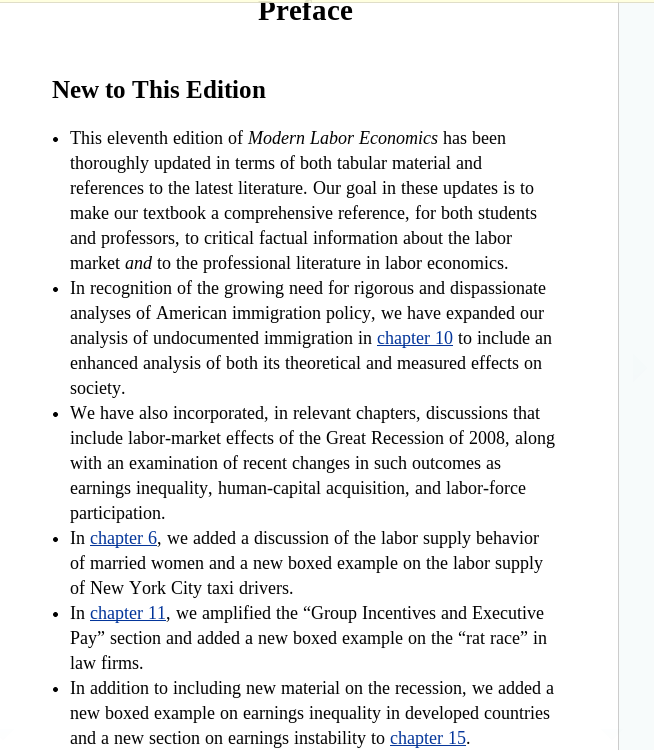
\includegraphics[height=.7\textheight]{EhrenbergSmith-preface-11.png}
\end{frame}

\begin{frame}{Principal idea}
\begin{columns}

\begin{column}{.48\textwidth}
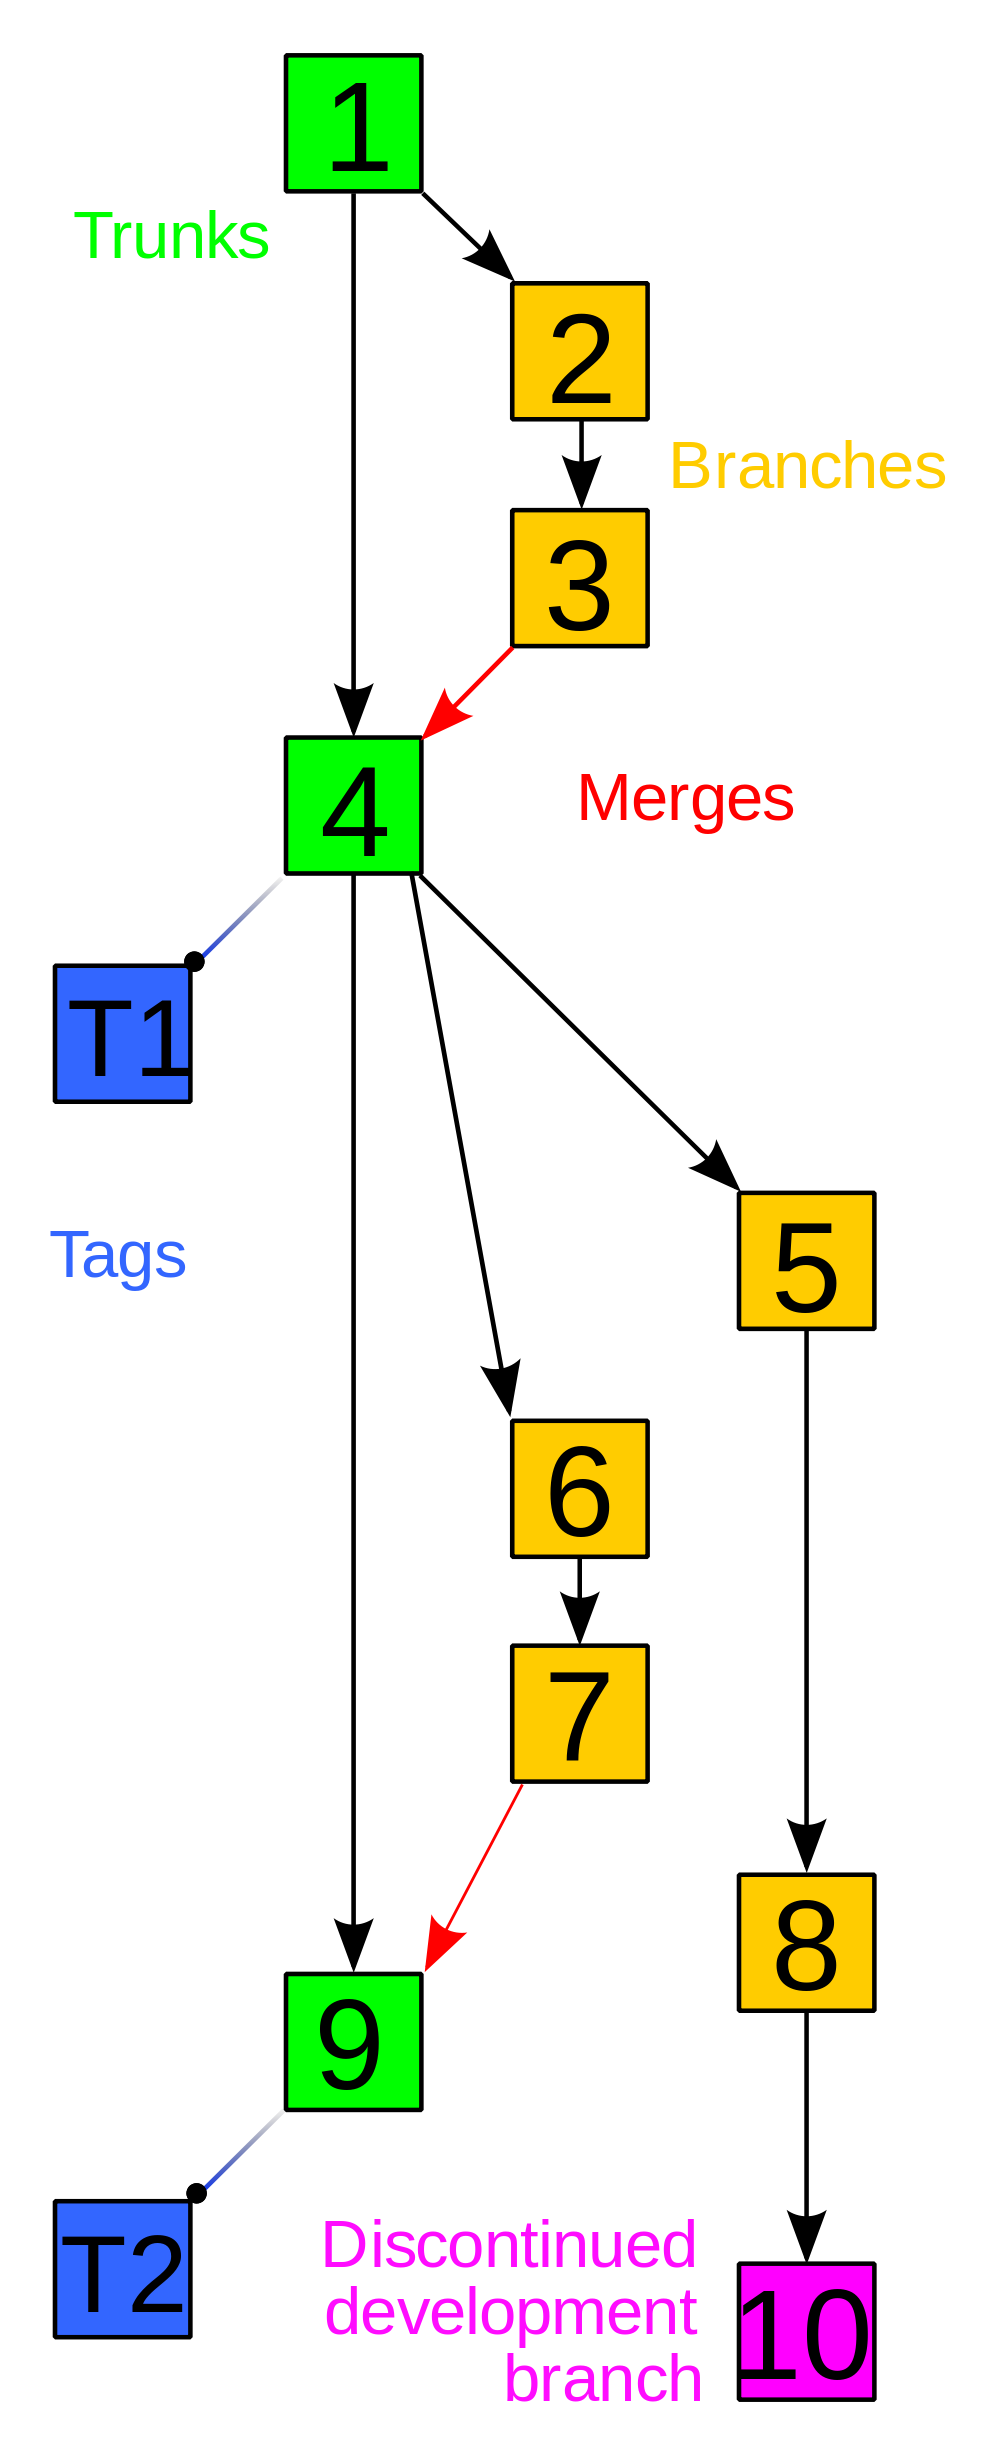
\includegraphics[height=.7\textheight]{Revision_controlled_project_visualization-2010-24-02.png}
\end{column}
\hfill
\begin{column}{.48\textwidth}
\begin{itemize}[<+->]
\item[1] First edition
\item[4] Second edition
\item[5] Start of work on a Canadian edition
\item[6] Start of work on the next US edition
\item[9] Third edition
\item[10] First Canadian edition
\end{itemize}
\end{column}
\end{columns}
\end{frame}

\begin{frame}{Two major types of version-management}
\begin{block}{Centralized model}
Server-client approach, editors check out a copy, modify it, and check it back in. Multiple editors:
\begin{itemize}
\item \textit{File locking}: only one person can check out any given file
\item \textit{Version merging}: discrepancies are handled upon checkin
\end{itemize}
\end{block}
\pause
\begin{block}{Distributed model}
There is no central server (prescribed by software). Every editor has a full copy of all version, synchronisation occurs by exchanging patches.
\end{block}
\end{frame}


\begin{frame}{Focus in this class}
We will focus on one system primarily, and mention a second one:
\begin{itemize}
\item Subversion (centralized)
\begin{itemize}
\item[Windows] \href{http://tortoisesvn.tigris.org/}{TortoiseSVN} (free)
\item[OSX] \href{http://versionsapp.com/}{Versions} (\$), \href{http://developer.apple.com/xcode/}{Xcode} (free)
\end{itemize}
\item Git (decentralized)
\end{itemize}
\end{frame}



\subsubsection{Quickstart on subversion}
\begin{frame}[fragile]{Quickstart on SSG/ECCO}
The following really quick tutorial can be run on SSG or on your own computer, if you already have the software installed.
\begin{lstlisting}[language=bash,numbers=none]
ssh NETID@ssg.vrdc.cornell.edu
Last login: Mon Aug 19 15:43:33 2013 from lv39-ws.ilr.cornell.edu
----------------------------------------------------------------------
Welcome to the Social Science Gateway (SSG),
for help, send email to ssg-help@cac.cornell.edu
----------------------------------------------------------------------
ssg:~> svn help
usage: svn <subcommand> [options] [args]
Subversion command-line client, version 1.6.6.
Type 'svn help <subcommand>' for help on a specific subcommand.
Type 'svn --version' to see the program version and RA modules
  or 'svn --version --quiet' to see just the version number.

Most subcommands take file and/or directory arguments, recursing
on the directories.  If no arguments are supplied to such a
command, it recurses on the current directory (inclusive) by default.

Available subcommands:
   add
   blame (praise, annotate, ann)
   cat
[snip]
\end{lstlisting}
\end{frame}

\lstset{language=bash,numbers=none}
\begin{frame}[fragile]{Quickstart Step 1}
Let's create a place to work
\begin{lstlisting}
mkdir Workspace
cd Workspace
\end{lstlisting}
\pause
Check out a version of the code:
\begin{lstlisting}
> svn co http://repository.vrdc.cornell.edu/public/test
A    test/test.3
A    test/test.4
A    test/releases
A    test/trunk
A    test/trunk/bls
[snip]
A    test/test.1
Checked out revision 23.
> 
\end{lstlisting}
\small
\begin{description}
\item[Checkout] 
To \textit{check out} (or \textit{co}) is to create a local working copy from the repository. A user may specify a specific revision or obtain the latest. The term 'checkout' can also be used as a noun to describe the working copy. 
\end{description}
\end{frame}


\begin{frame}[fragile]{Quickstart 2}
Using your favorite editor, modify a file:
\begin{lstlisting}
> cd test
> vi test.1
\end{lstlisting}
\pause
Verify the state of the repsository
\begin{lstlisting}
> svn status
M       test.1
\end{lstlisting}
\pause Let's also add a file:
\begin{lstlisting}
> vi test.today
> svn status
?       test.today
M       test.1
\end{lstlisting}
The question mark indicates that the file is not (yet) versioned.
\end{frame}



\begin{frame}[fragile]{Quickstart 3}
Add the unversioned file to Subversion tracking
\begin{lstlisting}
> svn add  test.today
A         test.today
> svn status
M       test.1
A       test.today
\end{lstlisting}
\pause
Now we can commit our changes
\begin{lstlisting}
> svn commit
[editor pops up]
Sending        test.1
Adding         test.today
Transmitting file data ..
Committed revision 24.
\end{lstlisting}
\small
\begin{description}
\item[Commit] 
To \textit{commit} (\textit{check in}, \textit{ci}) is to write or merge the changes made in the working copy back to the repository. The terms 'commit' and 'checkin' can also be used as nouns to describe the new revision that is created as a result of committing.
\end{description}
\end{frame}



\begin{frame}{Additional things you will want to learn}
\begin{block}{Manipulating files}
\begin{itemize}
\item \texttt{svn mv} (vs regular Linux mv or cut-and-paste)
\item Reverting changes (\texttt{svn revert} before a commit, more complicated after a commit)
\item Merging changes (\texttt{svn merge})
\item Inspecting logs (\texttt{svn log})
\item Identifying changes relative to previous revisions (\texttt{svn diff})
\end{itemize}
\end{block}
\end{frame}


\begin{frame}{THE reference for Subversion}
\begin{center}
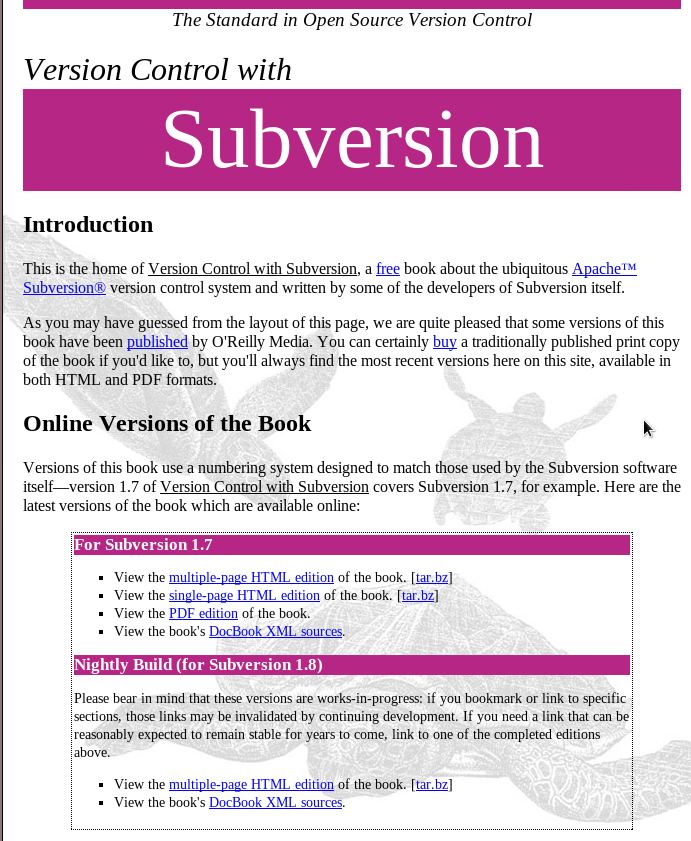
\includegraphics[height=0.7\textheight]{./svn-book}\newline\Large
\href{http://svnbook.red-bean.com/}{svnbook.red-bean.com}
\end{center}
\end{frame}


\begin{frame}{Learning more}
\begin{block}{A longer tutorial}
A longer tutorial (focussing on a complex project setup) is available at \href{http://www.vrdc.cornell.edu/computing-for-economists/web/COMPUTER_Subversion_LongTutorial.pdf}{the course website}.
\end{block}
\end{frame}









\subsection{Tracking history}
\begin{frame}{Tracking history}
\begin{block}{What happened? And who did what?}
One of the key advantages of using version control systems is ... to control versions.
\begin{itemize}
\item Straightforward to view multiple versions of a file (assuming proper usage)
\item Possibility to view who changed what (``blame'' or ``annotate'')
\end{itemize}
\end{block}
\end{frame}

\begin{frame}{Tracking using web interfaces: SVN}
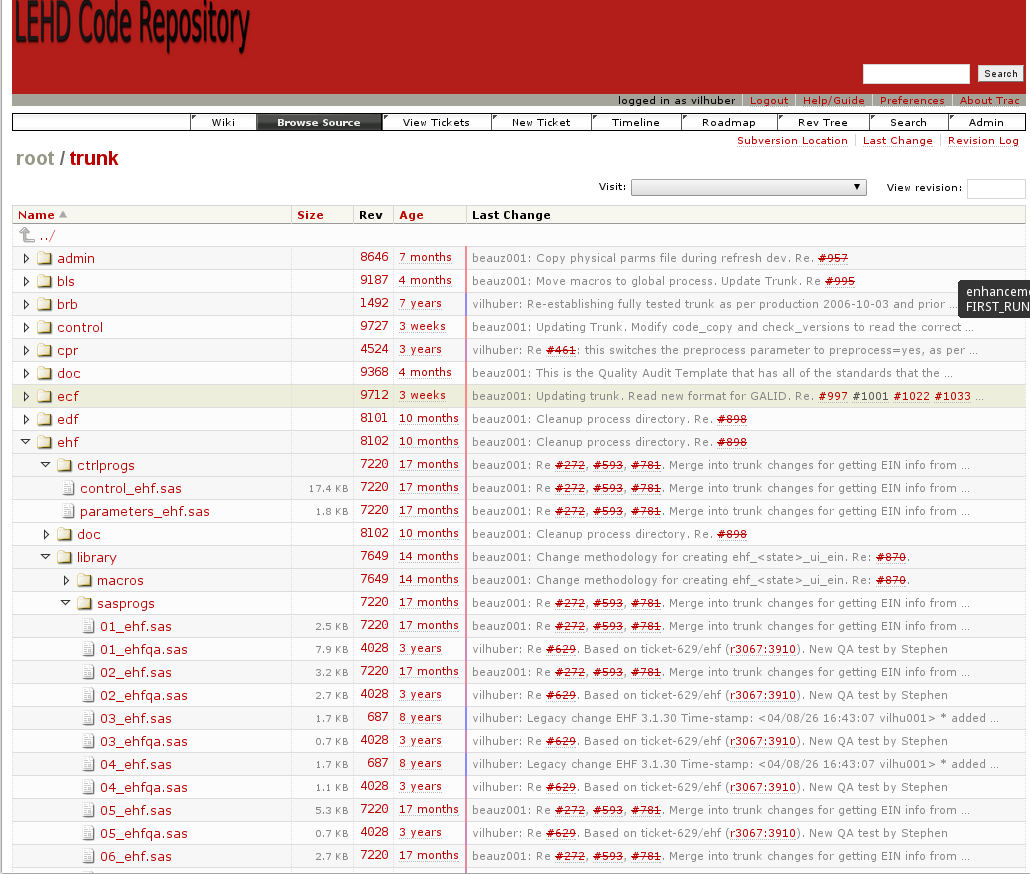
\includegraphics[width=.9\textwidth]{trac-svn-view1.png}
\end{frame}

\begin{frame}{Tracking using web interfaces: SVN}
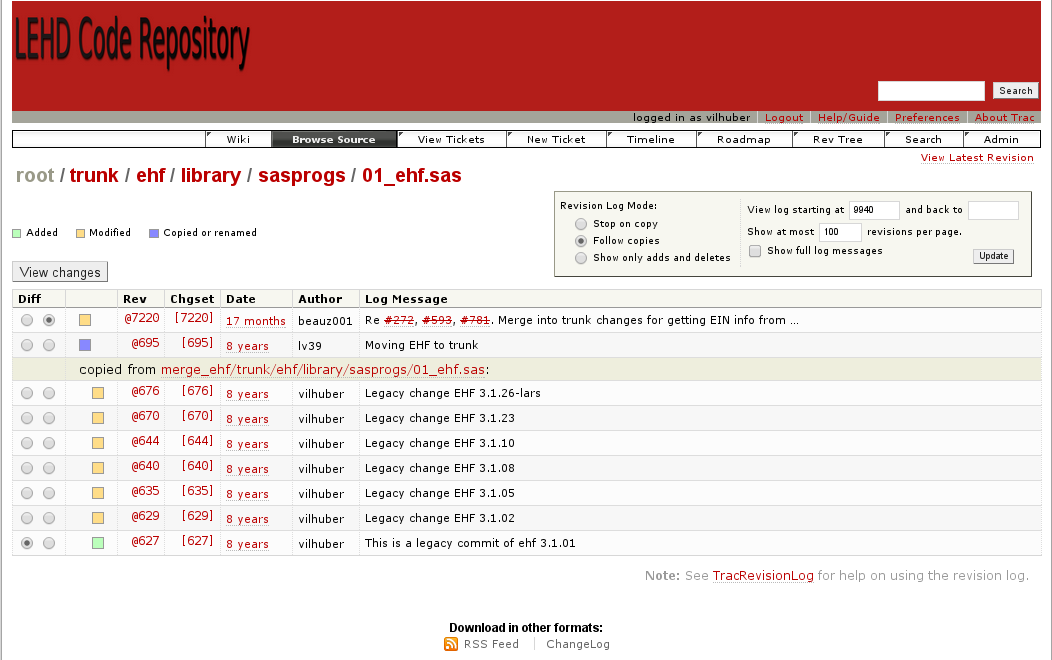
\includegraphics[width=.9\textwidth]{trac-svn-view2.png}
\end{frame}

\begin{frame}{Tracking using web interfaces: SVN}
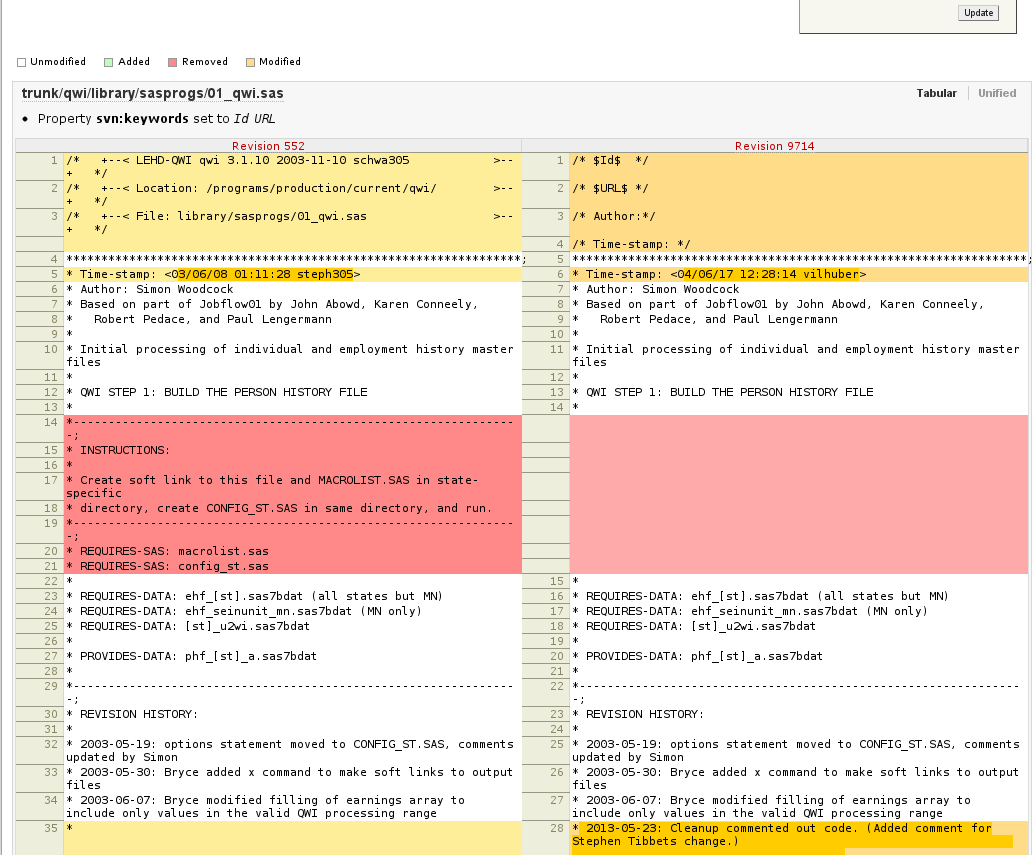
\includegraphics[width=.9\textwidth]{trac-svn-view3.png}
\end{frame}

\begin{frame}{Tracking using web interfaces: SVN}
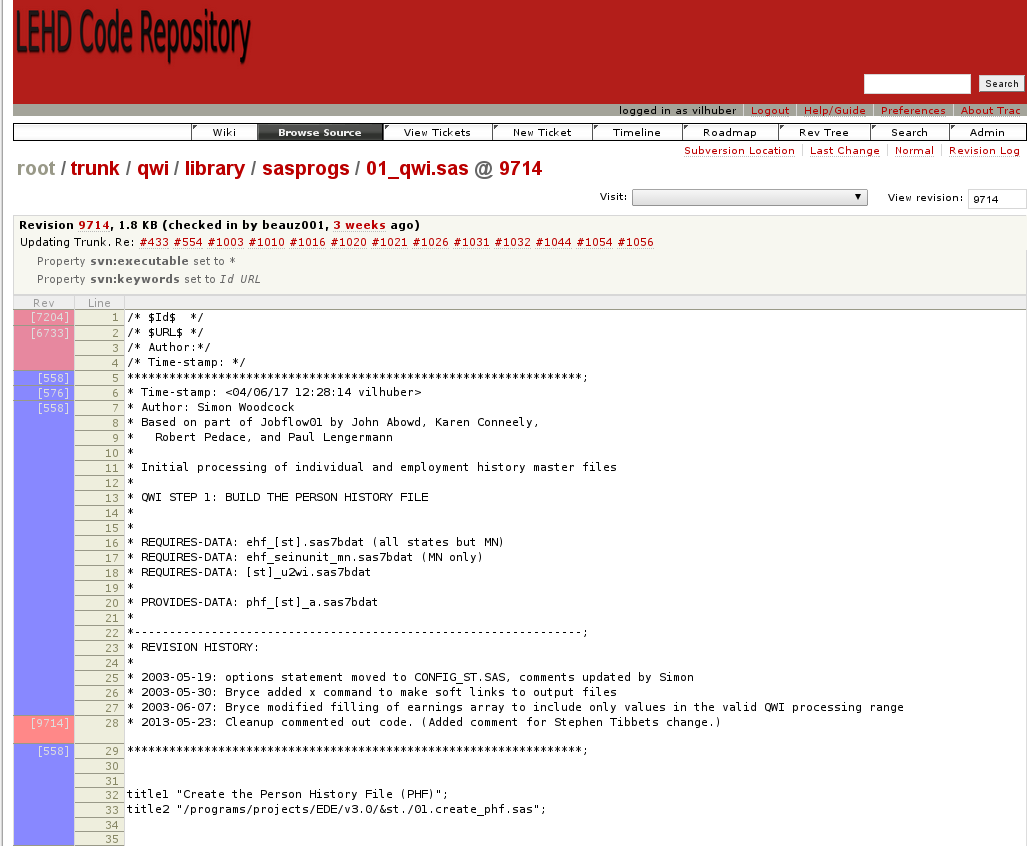
\includegraphics[width=.9\textwidth]{trac-svn-view4.png}
\end{frame}

\begin{frame}{Tracking using web interfaces: SVN}
\begin{block}{Including our demo change}
\href{http://repository.vrdc.cornell.edu/websvn/}{VRDC repository viewer}
\end{block}
\end{frame}


\begin{frame}{Tracking using web interfaces: git}
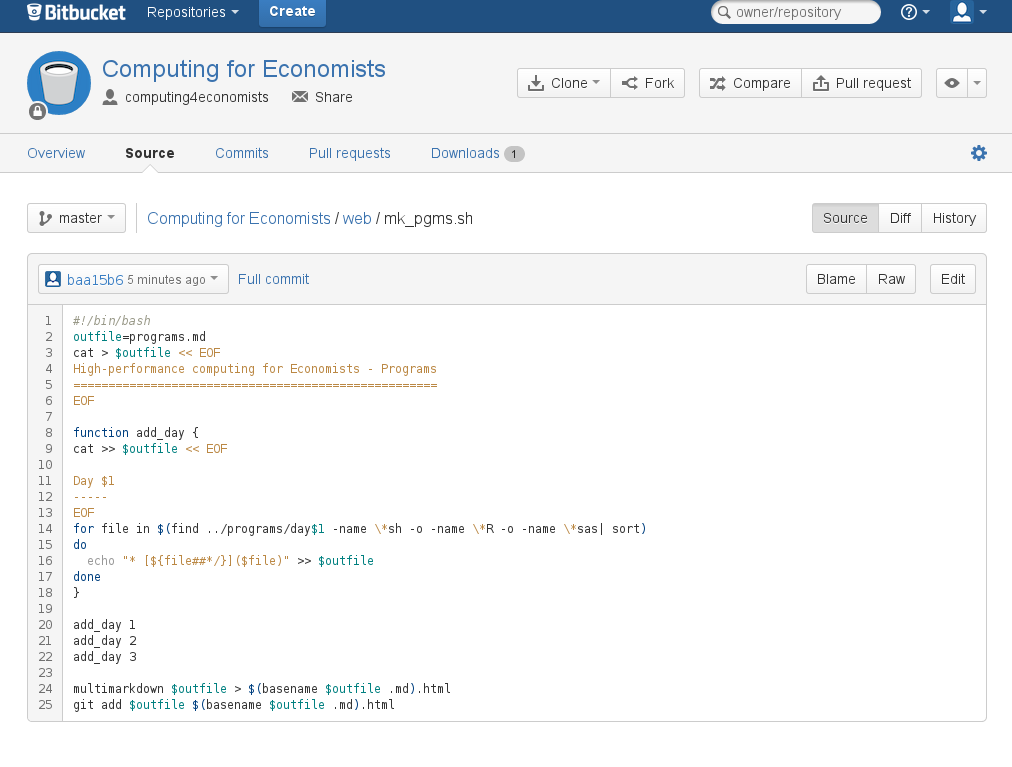
\includegraphics[width=.9\textwidth]{git-view1.png}
\end{frame}

\begin{frame}{Tracking using web interfaces: git}
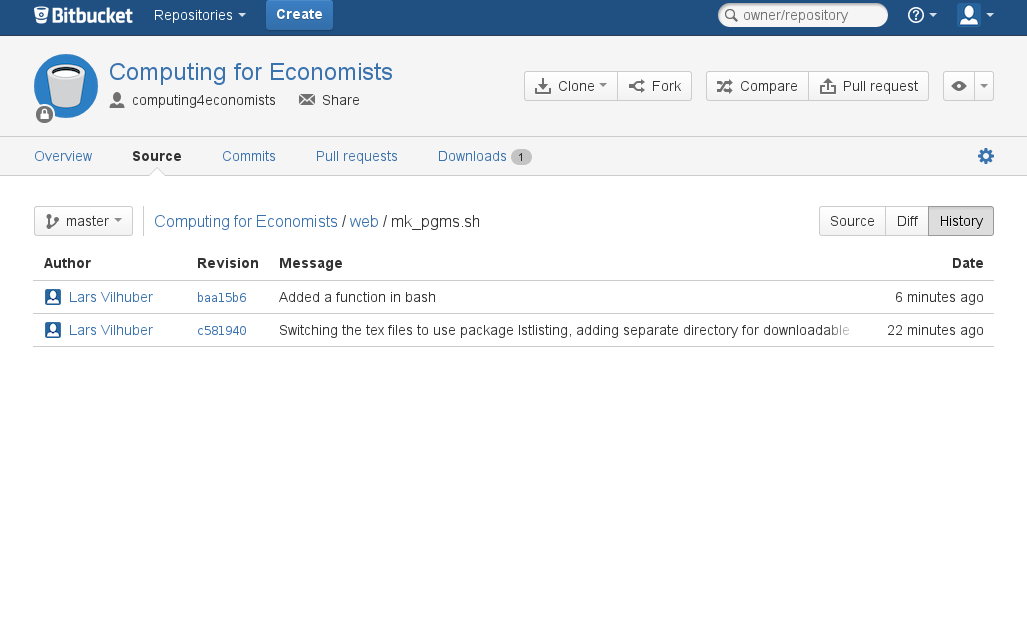
\includegraphics[width=.9\textwidth]{git-view2.png}
\end{frame}

\begin{frame}{Tracking using web interfaces: git}
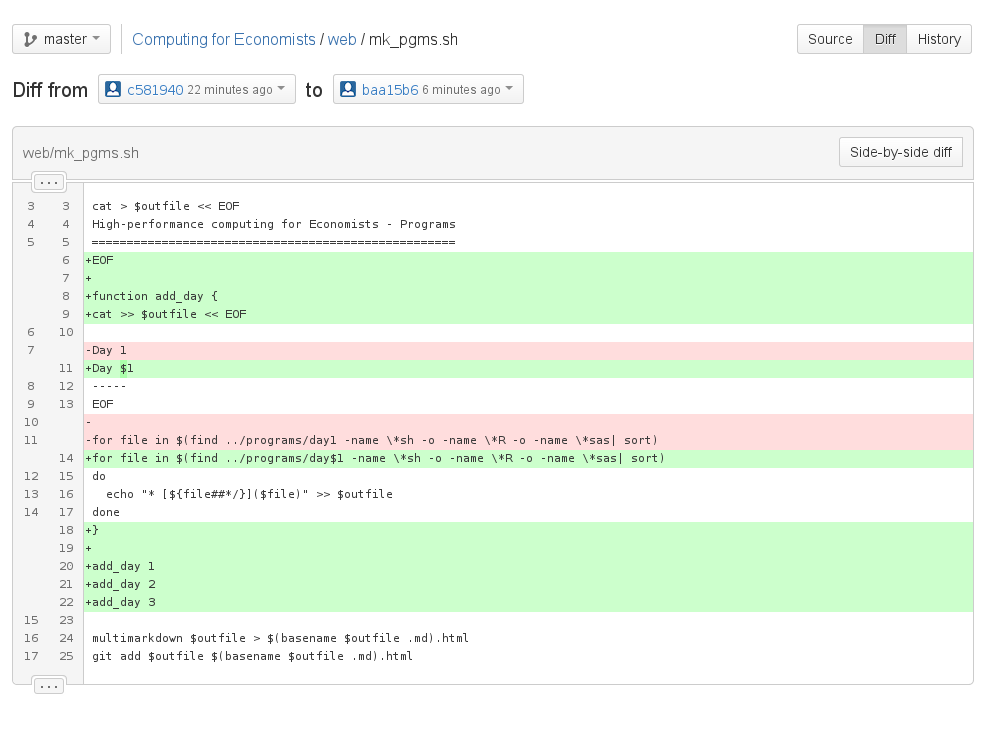
\includegraphics[width=.9\textwidth]{git-view3.png}
\end{frame}


\subsection{Comparing systems}
\begin{frame}[fragile]{Subversion vs. Git}
\small
incomplete
\begin{block}{Checking out a subdirectory}
\begin{columns}
\begin{column}{.48\textwidth}
\color{red}\rule{\linewidth}{4pt}

SVN
\end{column}%
\hfill%
\begin{column}{.48\textwidth}
\color{blue}\rule{\linewidth}{4pt}

GIT
\end{column}%
\end{columns}
\begin{columns}
\begin{column}{.48\textwidth}
\color{red}
\begin{lstlisting}
svn co ${URL}/sub/directory (name)
\end{lstlisting}
\end{column}%
\hfill%
\begin{column}{.48\textwidth}
\color{blue}\tiny
\begin{lstlisting}
mkdir <repo> && cd <repo>
git init
git remote add -f <name> <url>
git config core.sparsecheckout  true
echo some/dir/ >> .git/info/sparse-checkout
echo another/sub/tree >>  .git/info/sparse-checkout
git pull <remote> <branch>
\end{lstlisting}
{\tiny Source: \href{http://jasonkarns.com/blog/subdirectory-checkouts-with-git-sparse-checkout/}{here}}
\end{column}%

\end{columns}
\end{block}
\end{frame}


\begin{frame}{VCS infrastructure}
\begin{block}{At Cornell}
\href{https://forge.cornell.edu/sf/sfmain/do/home}{Cornell Sourceforge} (see \href{http://www.it.cornell.edu/services/subversion/howto/create.cfm}{instructions on how to create})
\end{block}
\begin{block}{Elsewhere}
\begin{itemize}
\item \href{http://app.cloudforge.com}{CloudForge} (free for personal use)
\item \href{https://github.com/plans}{GitHub} (Git, subversion, free for open-source)
\item \href{http://bitbucket.org/}{BitBucket} (Git, no subversion, free for academic users)
\item Roll your own: very simple webserver setup for Subversion, no server required for Git on your PC
\end{itemize}
\end{block}
\end{frame}




\section{Subroutines}
\begin{frame}
\href{day1-3.pdf}{Next section}
\end{frame}

\end{document}